\section{Neural Networks as Function Approximators}
\label{ch1:sec3}

Artificial intelligence deals with the automation of intelligent behaviour, which can be understood as the intelligence displayed by machines. Artificial intelligence further refers to the attempt to emulate certain decision-making structures of humans by, for example, building and programming a computer in such a way that it can handle problems relatively independently. Today, artificial intelligence is a thriving field with many practical applications and active research topics. Many applications involve deriving a general rule from a set of data, which is called machine learning. Artificial intelligence has recently made great progress in the field of artificial neural networks, which are roughly inspired by the structure of the human brain. These are artificially simulated on the computer and can be used as universal function approximators. \\
In this section we describe artificial neural networks, usually just called neural networks, which are computing systems inspired by the biological neural networks that constitute human brains. The original objective of the research field of artificial intelligence was to solve problems in the same way as the human brain would do, using a neural network approach. Today, neural networks can be used to model complex relationships between inputs and outputs or to find patterns in data. It has been shown that these systems can be used very well as classifiers as well as regressors or function approximators. \\
An artificial neural network is a collection of interconnected units called artificial neurons or just neurons that replicate biological neurons in a human brain, which are special cells in the nervous system that transmit information to other neurons through synapses. Each connection, like the synapses in a human brain, can transmit information, which can be understood as a signal, from one artificial neuron to another. The receiving neuron can process the signal, or even the signals, and then transmit signals to the downstream neurons that are connected to it. In common neural network types, the signal at a connection between artificial neurons is a real number, and the output of each artificial neuron is calculated by a non-linear function of the weighted sum of its inputs. Artificial neurons and their connections usually have a weight that changes during a learning process. The weight increases or decreases the strength of the signal at a connection, where a positive weight represents an excitatory connection, while a negative weight represents an inhibitory connection. \\
However, artificial neural networks are more about an abstraction of that information processing and less about replicating biological neurons or human brains. In 1958, the psychologist Frank Rosenblatt invented the first mathematical model for a single neuron, termed perceptron, in \cite{Rosenblatt:1958}, which was also the first artificial neural network. We want to use artificial neurons based on the perceptron and the neural networks constructed from them to approximate a variety of functions. \\
Let us describe how a single artificial neuron transforms a real-valued input into a 1-dimensional output, as illustrated in \cref{fig4}. Let there be $n$ real-valued input values summarized in a vector $(x_1, \ldots, x_n)^{\mathrm{T}} = x \in \mathbb{R}^n$. First, one forms a biased and weighted sum with the input values $x_1, \ldots, x_n$, which is nothing other than a linear combination, i.e. 
\begin{equation*}
    a = \sum^{n}_{i=1} w_i x_i + b = w^{\mathrm{T}} x + b,
\end{equation*}
where $(w_1, \ldots, w_n)^{\mathrm{T}} = w \in \mathbb{R}^n$ are called weights and $b \in \mathbb{R}$ is called bias. These weights and the bias are either predetermined or learned by the neuron itself through data (machine learning), but more on that later. The linear combination $a$ is called activation in the context of neural networks and a so-called activation function $\sigma \colon \mathbb{R} \to \mathbb{R}$ is applied to it, so that the output of that neuron becomes
\begin{equation*}
    y = \sigma \left( \sum^{n}_{i=1} w_i x_i + b \right) = \sigma \left( w^{\mathrm{T}} x + b \right) = \sigma(a).
\end{equation*}

\begin{figure}[H]
    \begin{center}
        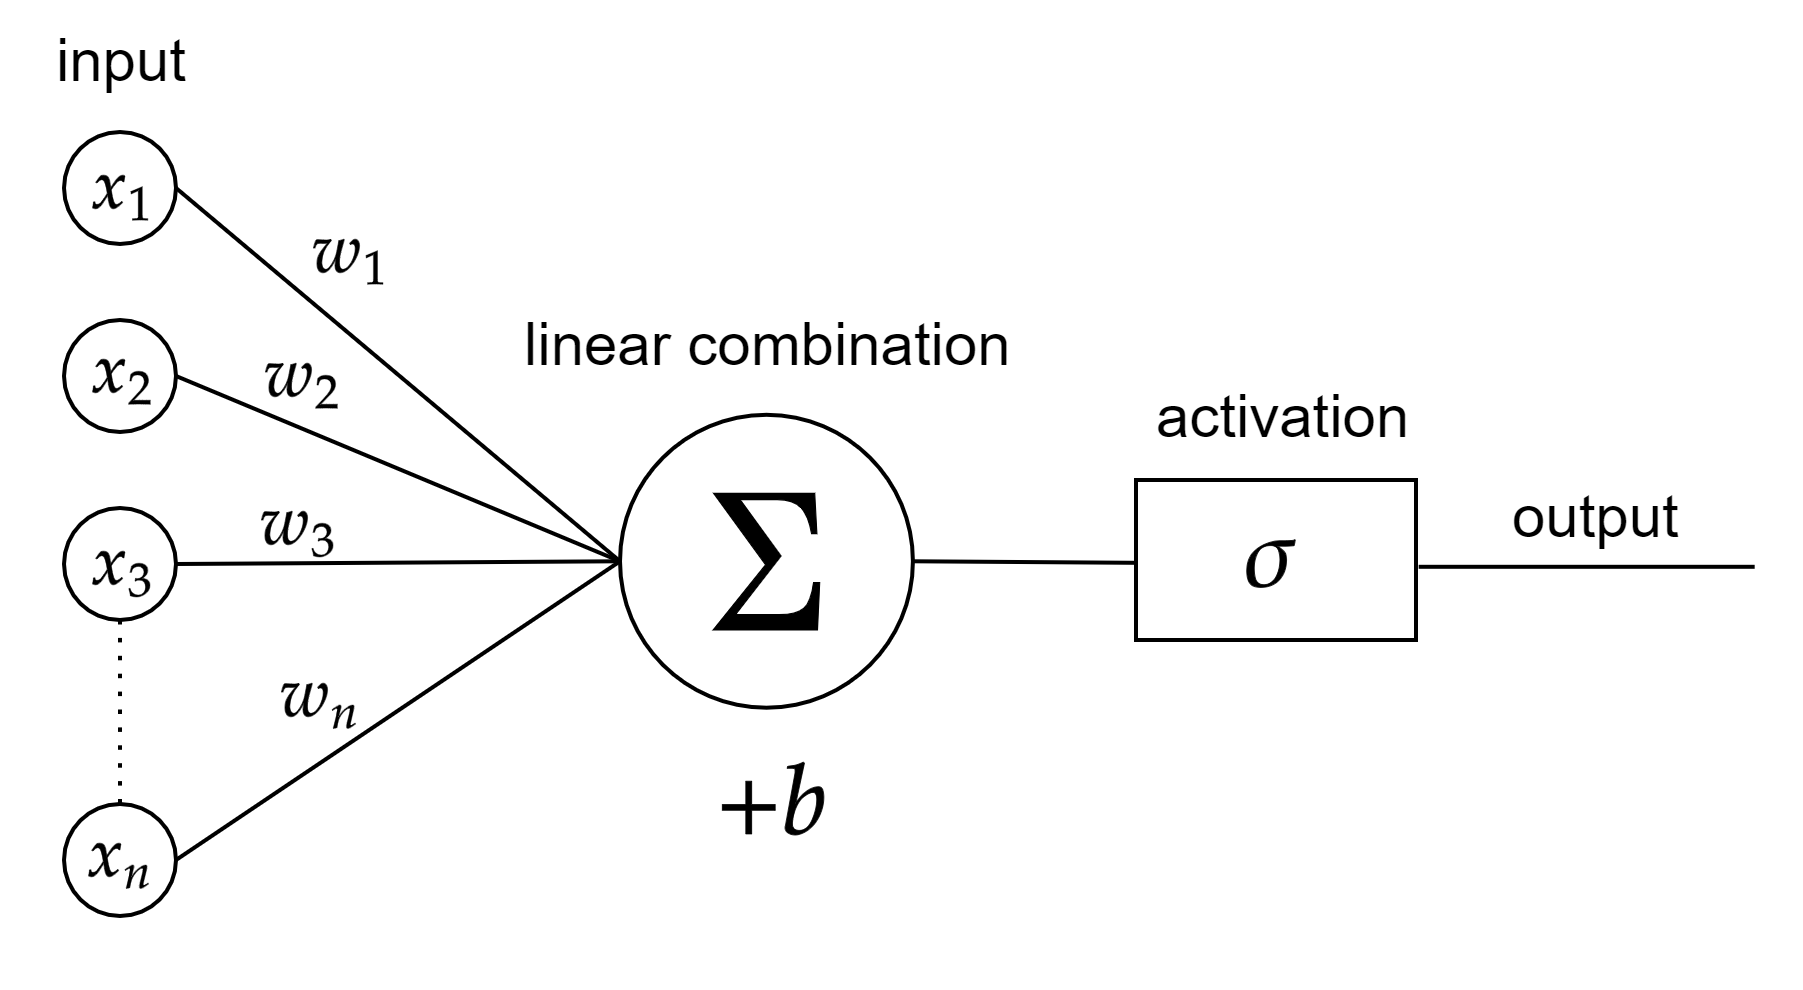
\includegraphics[scale=0.25]{img/diagram-20220205_1.png}
    \end{center}
    \caption{Illustration of the mathematical model of a single artificial neuron.}
    \label{fig4}
\end{figure}

The choice of activation function is determined by the nature of the input and the assumed distribution of the output. When the activation function is for example equal to the Heaviside step function, as described in \cite{Rosenblatt:1958}, i.e.
\begin{equation*}
    \sigma(x) = \begin{cases} 1 & \text{if } x \geq 0, \\ 0 & \text{if } x < 0, \end{cases}
\end{equation*}
then the artificial neuron coincides with a so-called linear support vector classifier, which is a mathematical method of pattern recognition that divides a set of objects into classes in such a way that the widest possible area around the class boundaries remains free of objects, see \cite[Chapter~7]{Bishop:2006}. \\
The task of the activation function is only to turn the linear combination of the input $a$ into a non-linear output $\sigma(a)$. Therefore, any non-linear, non-constant function can be an activation function, but those generally used are additionally monotone increasing, continuous, and at least piecewise smooth. At present, the most popular activation function is the rectified linear unit, abbreviated ReLU, \cref{ReLU}. In recent decades, smoother activation functions have also been used, such as the sigmoid function, \cref{Sigmoid}, or the hyperbolic tangent function, \cref{TanH}, \cite[p.~3]{LeCunBengioHinton:2015}.
\begin{align}
    \sigma(y) &=\max \{y, 0\} & & \text{ rectified linear unit (ReLU) } \label{ReLU} \\
    \sigma(y) &=\frac{1}{1+\exp (-y)} & & \text{ sigmoid } \label{Sigmoid} \\
    \sigma(y) &=\tanh (y)=\frac{\exp (y)-\exp (-y)}{\exp (y)+\exp (-y)} & & \text{ hyperbolic tangent } \label{TanH}
\end{align}

Unfortunately, a single neuron is incapable of both producing a multi-dimensional output and approximating any reasonably complicated function. This led to the creation of networks of artificial neurons, known as (artificial) neural networks. There are many different types of neural networks, which differ in their so-called architecture. This specifies how the neurons are organised, what activation functions are used and what other mathematical operations occur. Often a certain type of neural network is particularly suitable for a specific problem to be solved. A combination of different networks for solving a problem is also possible. \\
In the following, we focus on the best known and one of the most important types of neural networks, which form a specific class of neural networks that have proven most effective in practice, namely (deep) feed-forward neural networks, abbreviated FNNs. In these neuronal networks, the neurons are organized in multiple layers and neurons of one layer connect only to neurons of the immediately following layer. This means that the outputs of the neurons of one layer is utilized as inputs to the neurons of the following layer. This also describes the term feed-forward, which means that the information only flows in one direction, forwards. There are no backward connections in which outputs of one layer are fed back into itself. When FNNs are extended to include backward connections, they are called recurrent neural networks. Between the neurons of two layers, multiple connection patterns are possible. FNNs are in general fully connected, which means that the output of each neuron in one layer would be passed to all neurons in the following layer. FNNs are also known as multilayer perceptrons, although this name can be misleading as the artificial neurons are usually not the perceptrons as introduced in \cite{Rosenblatt:1958}. \\
We now describe how FNNs can be modelled in mathematical terms. We assume that we have $L \in \mathbb{N}$ layers of artificial neurons. We use $n_l \in \mathbb{N}$ to denote the number of neurons in layer $1 \leq l \leq L$. These numbers describe the topology of an FNN, the number of layers is called depth and the maximum number of neurons in a layer is called width of an FNN. This is why we also speak of deep feed-forward networks, as they can often have multiple layers. \\
To simplify the notation of FNNs, we introduce a so-called input layer with $l=0$, which only receives the external data $x$. It is the first layer of the network and does not change the input $x$ in any way. The number of neurons in this layer corresponds to the dimension of the input, i.e. $x \in \mathbb{R}^{n_{0}}$. From now on, we will refer to the last layer $l = L$ of a FNN, which produces the ultimate result, as the output layer. The number of neurons in this layer is equal to the dimension that the desired output should have, i.e. $y \in \mathbb{R}^{n_{L}}$. If an FNN has more than one layer, i.e. $L>1$, we refer to all layers between the input layer and the output layer as hidden layers. If the FNN does not have one hidden layer, it is called a single layer network because only the output layer $L=1$ processes the information. \\
We consider the information processing of a single layer $1 \leq l \leq L$. As input, each of the $n_l$ neurons in layer $l$ receives the output $x^{l-1} \in \mathbb{R}^{n_{l-1}}$ of the $n_{l-1}$ neurons in the previous layer $l-1$. Each neuron in layer $l$ has its own weight vector $w_i \in \mathbb{R}^{n_{l-1}}$, $i = 1, \ldots, n_l$. The weights of all $n_l$ neurons in layer $l$ can be conveniently organized into a matrix $W^l \in \mathbb{R}^{n_l \times n_{l-1}}$, where the $i$-th row is the transposed weight vector, $w^{\mathrm{T}}_i$, of the $i$-th neuron. We summarize the $n_l$ biases of the $n_l$ neurons into a vector $b \in \mathbb{R}^{n_l}$. The input $x^{l-1}$ is now linearly combined $n_l$ times with the weights and biases of the $n_l$ neurons of layer $l$ via 
\begin{equation}
    \label{propagation function}
    a^l = W^l x^{l-1} + b^l \in \mathbb{R}^{n_l}.
\end{equation}
We call \cref{propagation function} propagation function of layer $l$. \\
The same activation function is used in all neurons of layer $l$, which is why we define the activation function $\sigma \colon \mathbb{R} \to \mathbb{R}$ for vector-valued input values $a \in \mathbb{R}^{n_l}$ by applying it component-wise:
\begin{equation*}
    \sigma_l \colon \mathbb{R}^{n_l} \ni a^l \mapsto \sigma_l (a^l) \coloneqq \left(
        \begin{array}
            {c} \sigma_l \left( a^l_{1} \right) \\
            \vdots \\
            \sigma_l \left( a^l_{n_l} \right)
        \end{array}
        \right) \in \mathbb{R}^{n_l}.
\end{equation*}
We note that the activation function $\sigma_l$ can vary from layer to layer, which is why we indicate the dependency with the index $l$. The complete transformation of the input $x^{l-1} \in \mathbb{R}^{n_{l-1}}$ in the $l$-th layer can then be written as
\begin{equation}
    \label{action layer}
    \mathbb{R}^{n^{l-1}} \ni \underbrace{x^{l-1}}_{\text{input of layer } l} \mapsto x^{l}\coloneqq \underbrace{\sigma_{l}\left( W^{l} x^{l-1} + b^{l} \right)}_{\text{output of layer } l}=: f^{l}_{\theta_l} \left( x^{l-1} \right) \in \mathbb{R}^{n^{l}}, 
\end{equation}
where $\theta_l = (W^{l}, b^{l})$. \\

\begin{figure}[H]
    \begin{center}
        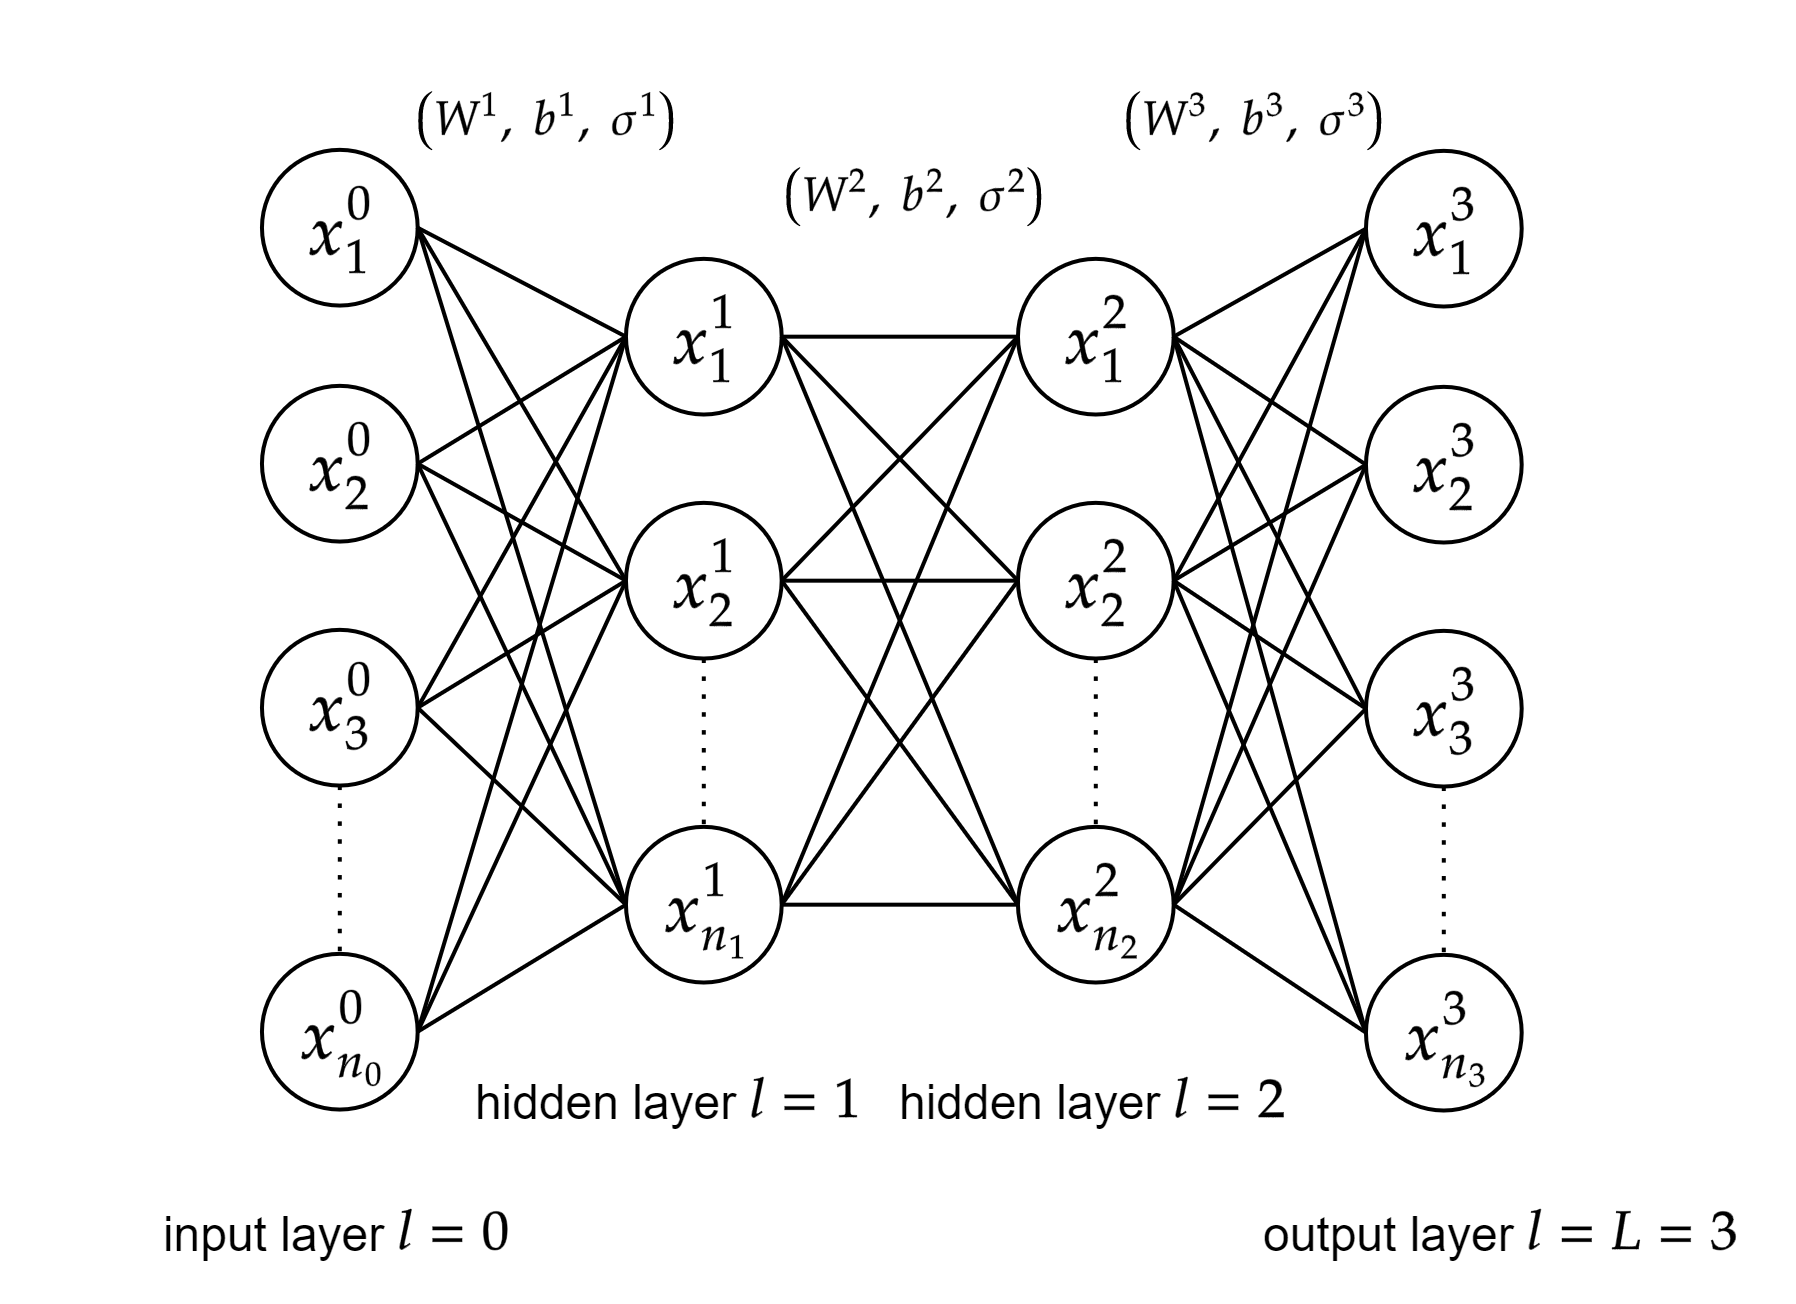
\includegraphics[scale=0.25]{img/diagram-20220206.png}
    \end{center}
    \caption{Illustration of a feed-forward neural network with $L=3$ layers.}
    \label{fig5}
\end{figure}

A feed-forward neural network consists of a composition of several of these layer-wise actions, \cref{action layer}, which are executed one after the other. Therefore, FNNs can be well represented as a directed acyclic graph (a directed graph with no directed cycles. We omit the arrows at the edges, since the flow direction of the information is in general always known.), where the neurons are represented as vertices and the connections of the neurons are represented as edges. The input layer $l=0$ is sometimes also represented as a layer of vertices. An example of an FNN is illustrated in \cref{fig5}, where the FNN has $L=3$ layers and therefore $2$ hidden layers. The mapping of the input $x = x^0 \in \mathbb{R}^{n_0}$ to the output $y = x^3 \in \mathbb{R}^{n_3}$ by the FNN is given by 
\begin{equation}
    \label{forward propagation of information}
    \begin{aligned}
        x^3 &=\sigma_{3} \left( W^{3} \sigma_{2} \left(  W^{2} \sigma_{1} \left( W^{1} x^{0}+b^{1}\right)+b^{2}\right)+b^{3}\right) \\
        & =f^{3}_{\theta_3} \left( f^{2}_{\theta_2} \left( f^{1}_{\theta_3} \left(x^{0} \right) \right) \right) \\
        & = f_{\theta} \left( x^{0}\right). \\
    \end{aligned}
\end{equation}
The process \cref{forward propagation of information} is called model prediction of the corresponding neural network and can be interpreted as a forward propagation of information through the layers of the network. In the following, we will identify the model prediction of a neural network with the subscript $\theta$, which constitutes the summary of all weights and biases (and other network-dependent parameters) of the network under consideration, i.e. $\theta = (W,b)$ with $W = \{ W^l \}_{l = 1, \ldots, L}$ and $b = \{ b^l \}_{l = 1, \ldots, L}$. From \cref{forward propagation of information} it is clear that the activation functions $\sigma_l$ should be non-linear. Otherwise, the output $x^L$ is a linear function of the input $x^0$ and all layers could be combined into one output layer. \\

We have seen how a FNN produces a non-linear multidimensional output from a multidimensional input. For a network to solve a problem such as approximating a function $f \colon \mathbb{R}^n \to \mathbb{R}^m$, the weights $W$ and biases $b$ need to be properly adjusted. This is what machine learning deals with, which is one of the most active areas of artificial intelligence. Machine learning is a generic term for the artificial generation of knowledge from experience: a neural network learns from examples that are given as a data set and can generalise them after a so-called learning phase. Neural networks do not simply learn the examples, but recognise patterns and regularities in the data. Deep learning is part of a broader family of machine learning methods that uses deep neural networks, abbreviated DNNs, to build out a comprehensive internal structure so that complex non-linear relationships can be modelled. DNNs are usually FNNs with a very high depth, i.e. with numerous hidden layers that perform different types of transformations on their input. The more complex the problem to be solved with the help of the neural network is, the more layers are needed. This number of many layers means that a lot of parameters, which are the entries of the weight matrices $W^l \in \mathbb{R}^{n_l \times n_{l-1}}$ and of the bias vectors $b^l \in \mathbb{R}^{n_l}$, have to be learned in a FNN, that is
\begin{equation*}
    \underbrace{n_0 \cdot n_1 + \ldots + n_{L-1} \cdot n_L}_{\text{weights}} + \underbrace{n_0 + \ldots + n_L}_{\text{biases}}.
\end{equation*}
The learning through data of these deep networks is called deep learning. Machine learning approaches are traditionally divided into three major categories, depending on the type of data available to the neural network: supervised learning, unsupervised learning and reinforcement learning, see \cite[pp.~1-3]{Bishop:2006}. We focus on the first two here. \\
Suppose we want to approximate a map
\begin{equation*}
    f \colon \mathbb{R}^n \to \mathbb{R}^m
\end{equation*}
with a FNN. In an supervised learning approach, it is assumed that a so-called training data set $\{ (x_i, y_i) \}_{i = 1, \ldots, N}$ is given, consisting of ordered pairs of inputs $x_i \in \mathbb{R}^n$ and desired output values $y_i \in \mathbb{R}^m$ of the function $f$ to be approximated, i.e. $y_i = f(x_i)$. The idea of supervised learning is to confront the neural network $f_{\theta}$, which is to approximate the function $f$, with the correct function value $y_i$ for an input value $x_i$. The goal is to train the neural network $f_{\theta}$ to make associations after several computations with different inputs $x_i$ and outputs $y_i$, so that the network $f_{\theta}$ approximates the function $f$ well to a certain degree. For this purpose, a cost function is defined that compares the desired output values $y_i$ with the outputs produced by the network $f_{\theta}(x_i)$ with the corresponding inputs $x_i$. This is generally achieved by using the so-called mean-squared-error, abbreviated $MSE$, which is the average squared difference between the generated values $f_{\theta}(x_i)$ and the actual values $y_i$. One then tries, with the help of a learning algorithm, to choose the weights and biases $\theta = (W, b) = (\{ W^l \}, \{ b^l \})_{l = 1, \ldots, L}$ such that the $MSE$ can be kept as small as possible over all data pairs $\{ (x_i, y_i) \}_{i = 1, \ldots, N}$. This can be defined as the following optimization problem:
\begin{equation}
    \label{supervised learning}
    \begin{gathered}
        \text{ Minimize } \underbrace{\frac{1}{N}}_{\text{normalization factor}} \sum_{i=1}^{N} \lVert \underbrace{ f_{\theta} \left(x_{i}\right)}_{\text{model prediction }} - \underbrace{y_{i}}_{\text{actual data }} \rVert^{2}_2 =  MSE(\{ (x_i, y_i) \}_{i = 1, \ldots, N}, \theta) \\
        \\
        \text{ where } \; \theta = (\{ W^l \}, \{ b^l \})_{l = 1, \ldots, L}, \; \; \left(W^{l}, b^{l}\right) \in \mathbb{R}^{n_l \times n_{l-1}} \times \mathbb{R}^{n_l}, \; \; l=1, \ldots, L .
    \end{gathered}
\end{equation}
\cref{supervised learning} is called a non-linear least-squares optimization problem. It is an unconstrained problem whose objective is generally non-convex. Of course, loss functions other than the $MSE$ can be used, but the $MSE$ has become the most common because of the differentiability it provides. \\
In an unsupervised learning approach, a training dataset is given only with input values, i.e. $\{ x_i \}_{i = 1, \ldots, N}$. In this machine learning approach, the networks try to recognise structures in the given input data. The networks therefore learn from data that has not been categorised in any way. Instead of responding to feedback, unsupervised learning methods identify commonalities in the data and respond based on the presence or absence of such commonalities. There are several methods of unsupervised learning. Again, there is the possibility of defining a cost function, which is passed an input value $x_i$ and the output generated by the network $f_{\theta}(x_i)$. The cost function depends on the problem and all a priori assumptions for the function $f$ to be approximated. However, a cost function can be very complicated, as its form depends on the problem at hand. One can again take the approach from \cref{supervised learning} and try to minimize the mean value of the cost function evaluated over all training inputs $\{ x_i \}_{i = 1, \ldots, N}$ and the output values generated by the network $\{ f_{\theta}(x_i) \}_{i = 1, \ldots, N}$ with respect to the weights $\{ W^l \}_{l = 1, \ldots, L}$ and biases $\{ b^l \}_{l = 1, \ldots, L}$. The unsupervised learning approach offers the advantage that only the input values must be available, which can be the case for many approximation problems. \\

Of course, the optimization problem in \cref{supervised learning} is not solved directly, but gradient-based optimization methods are generally used for this (which is why the term gradient-based learning is used for it, see e.g. \cite[p.~177]{GoodfellowBengioCourville:2016}), such as the variants of the gradient descent method. These are iterative methods that approximate a solution of \cref{supervised learning}, simply expressed via 
\begin{equation}
    \label{Gradient Descent}
    \theta_{k+1} = \theta_k - t \cdot \nabla_{\theta_k} \left( \frac{1}{N}\sum_{i=1}^{N} \lVert f_{\theta_k} \left(x_{i}\right) - y_{i}\rVert^{2}_2 \right) = \theta_k - t \cdot \nabla_{\theta_k} MSE(\{ (x_i, y_i) \}_{i = 1, \ldots, N}, \theta_k),
\end{equation}
where $\theta_k \in \prod^L_{l=1}  \mathbb{R}^{n_l \times n_{l-1}} \times \mathbb{R}^{n_l}$ are the iterates in the search space and $t > 0$ is the so-called learning rate, which can either be given or calculated with the help of a line search method. In many cases the data set $\{ (x_i, y_i) \}_{i = 1, \ldots, N}$ is very large and because of the linearity of differentiation and because the gradient $\nabla_{\theta_k} MSE(\{ (x_i, y_i) \}_{i = 1, \ldots, N}, \theta_k)$ also consists of many components, one for each $W^l$ and $b^l$, an ordinary gradient descent method may be too exhaustive to use. This is remedied by the stochastic gradient descent method, abbreviated SGD, in which $\nabla_{\theta_k} MSE(\{ (x_i, y_i) \}_{i = 1, \ldots, N}, \theta_k)$ is approximated by the gradient evaluated at only one data pair $(x_j, y_j)$, which is randomly selected from $\{ (x_i, y_i) \}_{i = 1, \ldots, N}$ with uniform distribution, i.e. $\nabla_{\theta_k} MSE((x_j, y_j), \theta_k)$ is used as direction in \cref{Gradient Descent}. An extension of this is the so-called mini-batch SGD method, in which $\nabla_{\theta_k} MSE(\{ (x_i, y_i) \}_{i = 1, \ldots, N}, \theta_k)$ is approximated by the gradient evaluated at a randomly selected small subset  of the data $\{ (x_i, y_i) \}_{i = 1, \ldots, J} \subsetneq  \{ (x_i, y_i) \}_{i = 1, \ldots, N}$ with $J \ll N$, a so-called mini-batch, i.e. $\nabla_{\theta_k} MSE(\{ (x_i, y_i) \}_{i = 1, \ldots, J}, \theta_k)$ is used as direction in \cref{Gradient Descent}. Especially for high-dimensional optimization problems, this reduces the computational effort and leads to cheaper iterations in exchange for a lower convergence rate. Mini-batch SGD is the de facto standard in neural network training, see \cite[sections~5.9~+~8.3.1]{GoodfellowBengioCourville:2016}. \\
The gradient is calculated using back-propagation, a technique of automatic differentiation, which is a family of methods for efficiently and accurately evaluating derivatives of numerical functions expressed as computer programs. Automatic differentiation takes advantage of the fact that any computer program executes a sequence of elementary arithmetic operations, such as addition, subtraction, multiplication, etc., and elementary functions, such as $\exp$, $\log$, $\sin$, $\cos$, etc. By repeatedly applying the chain rule to these operations, derivatives of any order can be calculated automatically, with machine precision, see \cite{BaydinPearlmutterAndreyevich:2018}. Back-propagation is a special case of the so-called reverse mode of automatic differentiation. The name comes from the fact that back-propagation lets the information given by $MSE((x_i, y_i), \theta_k)$ for a fixed data pair $(x_i, y_i)$ flow backwards through the neural network in order to calculate $\nabla_{\theta_k} MSE((x_i, y_i), \theta_k)$. Back-propagation consists of two phases. First, the corresponding FNN $f_{\theta} \left(x_{i}\right)$ and the objective $MSE((x_i, y_i), \theta_k)$ is evaluated and certain data is stored. Then, this data is used to calculate $\nabla_{\theta_k} MSE((x_i, y_i), \theta_k)$ with respect to each weight matrix $W^l \in \mathbb{R}^{n_l \times n_{l-1}}$ and bias vector $b^l \in \mathbb{R}^{n_l}$ using the chain rule, calculating the gradient layer by layer and iterating backwards from the last layer $l=L$ to avoid redundant calculations of intermediate terms in the chain rule. Back-propagation is an inexpensive method and can be integrated into a gradient descent method without much effort, see \cite[section~6.5]{GoodfellowBengioCourville:2016}.\\

Deep neural networks could approximate in general any high-dimensional function if sufficient training data is available, see e.g. \cite{ArzaniDawson:2021}. Therefore, FNNs can be understood as universal approximators for vector-valued, measurable, especially continuous, functions if they are given suitable weights and biases, which was shown in the universal approximation theorem. The theorem refers to the ability of FNN with a single hidden layer with a finite number of neurons to approximate continuous functions. The first proof was published in \cite{Cybenko:1989} for sigmoid activation functions, \cref{Sigmoid}, and was generalised to feed-forward multi-layer architectures in \cite{Hornik:1991}. In \cite{SonodaMurata:2017} it was shown that the universal approximation also holds for unbounded activation functions such as ReLU, \cref{ReLU}. In \cite{HornikStinchcombeWhite:1990}, it was shown that the derivatives of the FNN can also approximate the derivatives of the function, which is approximated by the FNN, arbitrarily well. \cite{LuPuWangHuWang:2017} considered an universal approximation theorem for deep neural networks concerning the capacity of networks of finite width, where the depth is allowed to grow, and showed that if the width of a deep neural network with ReLU activation is strictly larger than the input dimension, the network can approximate any Lebesgue integrable function. Overall, this means that "any reasonable" function can be approximated with an arbitrary small error by an FNN with a suitable topology. Unfortunately, however, all the proofs are non-constructive in terms of the number of neurons required, the network topology, the weights and the biases. \\

Finally, there is the question of which type of neural network is best suited for which problem. Unfortunately, this question is difficult to answer. In general, one relies on the user's expertise in machine learning and their ability to decide on the right type of neural network based on the characteristics of the problem. The machine learning toolbox offers the so-called neural architecture search, abbreviated NAS, which is a technique for automating the creation of artificial neural networks. NAS is used to identify networks that match or outperform user-designed architectures, see \cite{ZophLe:2017}. NAS methods can be categorised by the search space, which defines the types of neural networks that can be designed and optimized, the search strategy, which specifies the approach used to explore the search space, and the performance estimation strategy, which evaluates the performance of a potential neural network based on its design without constructing and training it, \cite{ElskenMetzenHutter:2019}. Should the choice fall on an FNN, there is still the question of the correct topology of the FNN for the corresponding problem. This question is also very difficult to answer. But as mentioned above, a certain width or depth is necessary for a certain degree of approximation. Here, too, the large toolbox of machine learning offers a solution approach, which is called hyperparameter optimization. A hyperparameter is a constant parameter whose value is determined in advance before the learning phase starts. Examples of hyperparameters include of course the width and depth, the used activation functions as well as the connection patterns between the neurons. The values of some hyperparameters can be dependent on those of other hyperparameters, for example, the depth can depend on the width in a FNN. Choosing the right set of hyperparameters is extremely difficult, it is not unusual for the user to find these by trial and error. In machine learning, hyperparameter optimization concentrates on the problem of selecting a set of optimal hyperparameters that results in an optimal neural network that minimizes a predefined loss function given the data, see \cite{ClaesenDeMoor:2015}. The best known approaches in hyperparameter optimization are: The grid search, which is simply an exhaustive search through a manually defined subset of the space of hyperparameters in question. A grid search algorithm must be guided by a performance metric, which is usually measured by cross-validating the training set, see \cite{HsuChangLin:2003}. The random search, which replaces exhaustive enumeration of all combinations with random selection. It can outperform grid search, especially when only a small number of hyperparameters affect the final performance of the machine learning algorithm, see \cite{BergstraBengio:2012}. And the Bayesian optimization approach, where a probabilistic model of the function is created that maps the values of the hyperparameters to the target, which is evaluated against a validation set. By iteratively evaluating a promising hyperparameter configuration based on the current model and then updating that model, Bayesian optimization aims to collect observations that provide as much information as possible about that function and, in particular, about the location of the optimum. In practice, Bayesian optimization has been shown to produce better results with fewer evaluations compared to grid search and random search, as it is able to draw conclusions about the quality of the experiments before they are conducted, see \cite{SnoekLarochelleAdams:2012}.





% curse of dimensionality 
% Tensorflow
% Lernen ist aufwendigster Prozess von NN


